
\subsection{Architettura del Sistema}

Il sistema segue il pattern architetturale \textbf{Model-View-Controller (MVC)}, un'architettura software che separa la logica di presentazione, la logica di business e la gestione dei dati. Questa separazione consente una maggiore modularità e facilita la manutenzione e l'estendibilità del sistema. Le tre componenti principali sono:
\begin{figure}[H]
    \centering
    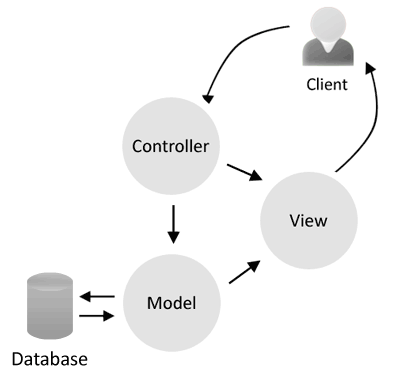
\includegraphics[scale=0.45]{images/mvc.png}
    \caption{M-V-C Pattern }
\end{figure}
\subsubsection{Model}
Il \textbf{Model} rappresenta la logica di business e la gestione dei dati. In questo sistema:
\begin{itemize}
    \item I dati sono memorizzati in un database relazionale \textbf{PostgreSQL}, scelto per la sua affidabilità e scalabilità.
    \item Il backend, implementato in \textbf{Spring Boot}, gestisce le operazioni sui dati attraverso un'architettura basata su servizi.
    \item I principali servizi includono:
    \begin{itemize}
        \item \textbf{Servizio Utente}: gestione della registrazione, autenticazione (tramite \textbf{JWT}) e gestione del profilo utente.
        \item \textbf{Servizio Gestione Spese}: esecuzione delle operazioni CRUD sulle spese degli utenti.
        \item \textbf{Servizio Gruppi}: creazione e gestione dei gruppi di utenti.
    \end{itemize}
    \item L'interazione con il database avviene tramite il \textbf{Data Access Layer}, basato su JPA e Hibernate.
\end{itemize}

\subsubsection{View}
La \textbf{View} è responsabile della presentazione dei dati all'utente e della gestione dell'interazione con il sistema. Nel nostro caso:
\begin{itemize}
    \item Il frontend è sviluppato utilizzando \textbf{Vue.js}, un framework JavaScript progressivo che permette lo sviluppo di interfacce utente reattive e modulari.
    \item Le chiamate API al backend vengono gestite tramite \textbf{Axios}, consentendo un flusso di dati asincrono tra client e server.
    \item L'autenticazione degli utenti è gestita tramite token \textbf{JWT}, che vengono memorizzati e inviati nelle richieste HTTP per garantire la sicurezza.
\end{itemize}

\subsubsection{Controller}
Il \textbf{Controller} funge da intermediario tra il Model e la View, gestendo le richieste utente e applicando la logica di business. In questo sistema:
\begin{itemize}
    \item Il backend espone un'API \textbf{RESTful} tramite Spring Boot, con endpoint per la gestione di utenti, spese e gruppi.
    \item Ogni richiesta HTTP viene elaborata da un controller dedicato, che interagisce con i servizi del Model per recuperare o aggiornare i dati.
    \item Le risposte sono restituite in formato JSON, consentendo una comunicazione fluida con il frontend.
\end{itemize}

\subsubsection{Flusso delle Richieste}
Il flusso di una tipica richiesta utente segue questi passi:
\begin{enumerate}
    \item L'utente interagisce con il frontend Vue.js tramite un'interfaccia web.
    \item Un'azione (es. login, aggiunta di una spesa) genera una richiesta HTTP verso il backend.
    \item Il \textbf{Controller} riceve la richiesta e invoca il servizio appropriato.
    \item Il \textbf{Model} esegue la logica di business e interagisce con il database per recuperare o aggiornare i dati.
    \item La risposta viene inviata al frontend in formato JSON.
    \item Il frontend aggiorna dinamicamente l'interfaccia utente con i nuovi dati.
\end{enumerate}
Questa architettura garantisce una chiara separazione delle responsabilità, facilitando lo sviluppo, la scalabilità e la manutenzione del sistema.

